\chapter{Literature Review}
\label{chap:literature_review}

% focused, concise
% supports the well-stated question
% identifies a gap
% reports and critiques current state of discourse
% critical
% adds value

% motivation

Given the aims identified in the introduction, this chapter investigates the existing work that can help us understand the \emph{framing} phenomenon, and how it is detected by automatic approaches, usually performed on single articles.
% how we can expand the current state of detection by using the information coming from other articles.
But, as mentioned previously, this type of analysis struggles to detect the framing when it is very subtle and manifests through techniques such as focusing on certain aspects, or selecting which details to include or omit, or even selecting a specific order inside a story~\cite{morstatter2018identifying}.
For these specific cases, it is very complicated to spot the signals of framing taking place, and we argue that both human and automated analysis would benefit from comparing different articles that talk about the same event but have different perspectives. %taking a look at other articles.

This multi-article knowledge requires introducing a second family of methods that aims at finding \emph{similarities} between articles, by using document and sentence representations, and to find which pieces appear in multiple documents. In this way the common ground can be identified, as well as the diversity in the information reported.
With this second family of methods we can see that for a certain event there are several articles which overlap in part, and some of them have unique pieces or specific words that differ from the others. But this analysis needs an interpretation framework that is able to describe the framing role of the choices done by each of the sources.

Exploring these two different fields of research, we can see that there is an intersection area that is not much explored, that is the analysis of framing differences. Given the differences identified by this second group of methods, we need to expand the framing analysis to work with multiple documents and understand why modifications in the text happen.
There are works that analyse this specific field, but using manual handcrafted analysis, that for example show how events are described from sources belonging to different political leanings. We want to target this specific area with an automated analysis.
%under the perspective of social science (manual analysis, not automated), and the automation of this type of analysis is an existing gap.

% structure

For these reasons, this chapter is structured in three parts: framing analysis of single documents (Section~\ref{sec:lit_framing}), similarities between multiple documents (Section~\ref{sec:lit_relationships}) and finally the point of contact between the two (Section~\ref{sec:lit_gap}), as our target niche.

% The structure of 2.1 and 2.2 is inside 2.1 and 2.2
% expanding on framing theories in Section~\ref{ssec:lit_framing_theory}, then moving to automated framing analysis in Section~\ref{ssec:lit_framing_auto}. Section~\ref{ssec:lit_framing_other} is providing some insights about related analyses that are quite related to framing (e.g., subjectivity, source bias and factuality) and Section~\ref{ssec:lit_framing_limit} exposes the limits of the single-article framing analysis.
% Then we move to the second area, that is ~\ref{sec:lit_relationships}: 
% We are considering two main research areas that are related to our problem: \textit{i)} framing analysis and \textit{ii)} analysis of similarities between documents.

\section{Framing}
\label{sec:lit_framing}

% definition
As we are using the term \emph{framing}, we need to define what we mean with it, because multiple definitions do exist.
% Before exploring the framing analysis area, we need to define what we mean with framing, because multiple definitions exist.
% - broad framing as perception of the world (goffman)
The broadest definition comes from \citet{goffman1974frame} who defines framing as how people organise experiences about the world.
% - semantic frames
Then we have the Frame Semantics~\cite{fillmore2006frame} that instead defines a frame as ``\textit{any system of concepts related in such a way that to understand any one of them you have to understand the whole structure in which it fits}''. This second definition goes into the direction of annotating sentences with units of meaning (semantics) that are evoked by specific words, e.g. FrameNet~\cite{baker1998berkeley}.

% - media framing
But the definition that we rely on, instead focuses on the power of media to present facts under a specific light: instead of focusing on \emph{what} is contained in a text (semantics), we focus on \emph{how} it is described.
This facet of the term can be seen in the work of
\citet{entman1993framing} that defines framing as ``\textit{select[ing] some aspects of a perceived reality and make them more salient in a communicating text}''.
Or from \citet{goffman1974frame} that describes framing as ``\textit{how a certain story is presented to shape mass opinion}''.
% some description and insight about how it is described
Using this connotation, framing becomes an additional layer on top of the factual information focusing on the presentation side, giving a structure (identifying problems, causes, resolutions) where each of the semantic elements is given a role to create a coherent story~\cite{pan1993framing}.

% difference with propaganda
Framing is used every day to influence the readers and make some messages pass more than others, and becomes really important in the political sphere where it is used as a propaganda technique to promote or demote candidates and ideologies by creating and sustaining narrative lines that coherently align with a specific communication goal.
% propaganda is targeted for a specific goal, framing instead is what is used to do propaganda. Framing exists also without propaganda
Although this is a very common use of framing, in day by day communication there is a lot of framing that can influence the readers even though there is not a clear propaganda target.

% ``the central organising themes ... that connect different semantic elements of a news story (headlines, quotes, leads, visual representations, and narrative structure) into a coherent whole to suggest what is an issue.''~\cite{pan1993framing}

% Structure of 2.1 (too much?)
% We expand in the following on \textit{i)} framing techniques, where we can see how previous research identified a set of concrete phenomena, then we move to practical framing detection models and finally to the identification of concepts that are very much related to framing but have an independent meaning.
% We are expanding on framing theories in Subection~\ref{ssec:lit_framing_theory}, then moving to automated framing analysis in Subection~\ref{ssec:lit_framing_auto}. Subection~\ref{ssec:lit_framing_other} is providing some insights about related analyses that are quite related to framing (e.g., subjectivity, source bias and factuality) and Subection~\ref{ssec:lit_framing_limit} exposes the limits of the single-article framing analysis.

\subsection{Framing techniques}
\label{ssec:lit_framing_theory}
% Framing theories and definitions
% framing: definition and theory

% We have a group of theoretical studies that define the concept of \textit{media framing}~\cite{gamson1989media,scheufele2007framing},

% concepts
Media framing, under the theoretical perspective, is composed of several concepts and processes~\cite{scheufele2007framing}.
% 1. frame building (how to fit articles into a broader coherent narrative that has been built)
\textit{Frame building} is the process of creating a narrative in which the articles can fit. It corresponds to defining the objectives of the communication in which several articles can be fitted coherently. Under this point of view the frames are the output of the societal, organisational, ideological, political and cultural contexts~\cite{scheufele1999framing}.
%~\cite{scheufele1999framing}
% It produces ``media frames'' that are embedded in the articles.
% 2. frame setting
Then there is the process of \textit{frame setting} that instead takes the frames as inputs and describes the transfer from the writer to the readers. How the document has been written creates the ``audience frames'': the reader is placed in a certain mental perspective. For this to happen, a big role is played by the selection of media coverage (which issues to cover or not, how to use emphasis)~\cite{iyengar1994anyone} and the specific use of language that conveys how to think and feel about an issue~\cite{bryant2012fundamentals}.
% % 3. individual level effects of framing
% And then there is the individual effects on the audience, in other words the internalisation (attribution of responsibilities, attitudes, behaviours).
Inside this process we can place the quite known \emph{agenda setting} theory~\cite{mccombs1972agenda} that describes the ability of news media to influence the importance of the topics, by selecting the information for the reader (what to think about, not how): % that is used to influence the relevance of a certain event:
the number of article that are published about each event is an indicator of this process, which can have an avalanche effect as lot of outlets want to have their piece on the same event too.
But the agenda setting can be seen also at a more fine-grained level: stories are made of details and different sources can emphasise them with different weights.

% and how it acts as an intermediary between the writers and the consumers of the news, via the processes of frame setting and individual-level effects on the public~\cite{scheufele1999framing} (diagram of media vs public and processes)

% Switching from abstract concepts and processes to more tangible, 
Framing is usually defined at macro and micro levels.
For the macro-level, usually, each article is associated with a set of media framing packages, which correspond to a central idea with a surrounding interpretive structure that gives meaning to an issue~\cite{gamson1989media}.
And then the micro-level analysis focuses on seeing how the defined frames come out from specific words, used as \textit{framing devices} (e.g., word choice, metaphors, catchphrases, use of contrast, quantification) and \textit{reasoning devices} (e.g., problem definition, cause, consequence, solution, action).
The macro-level labelling of framing (e.g., saying that a certain article is belonging to a specific narrative) is very difficult for automatic approaches because of different reasons. Firstly, it needs to be specific for every topic and story, it cannot encode all the possible positions with respect to all the possible issues. And it requires contextual knowledge of the events.
For these reasons, we want to focus more on the micro-level that instead targets the detection of \emph{techniques} that are used transversely to the specific topics. These framing techniques need to be simple to describe and capture punctual details.

% techniques described by others
From the literature many works describe and categorise framing techniques that can be seen on the micro-level. Here we have a list of the most important.
% the following techniques which try to capture the language of framing:

\begin{itemize}
    \item \textbf{Recurrent themes}: this technique is achieved by repeating and reinforcing certain themes in the articles, making the readers perceive certain topics more important than others because they appear more in the news. This is the direct manifestation of the agenda setting theory, where the press has the power to influence the importance of the issues.
    % , commonly known as ‘spin’~\cite{tsur2015frame} (e.g. health, energy, security, economy).
    This can be done on broad granularity, as analysed by different studies~\cite{tsur2015frame,card2015media}, where each document is associated with very wide media frames, not dependent on any specific topic (e.g., economics, politics, health, ...).
    % Economic, Capacity and resources, Morality, Fairness and equality, Legality, constitutionality and jurisprudence, Policy prescription and evaluation, Crime and punishment, Security and defense, Health and safety, Quality of life, Cultural identity, Public opinion, Political, External regulation and reputation, Other.
    Or other studies that investigate more on a more fine-grained level using hierarchical topic modelling to identify both issue-specific and generic frames~\cite{boydstun2013making}.
    This, however, is still limiting the ability to evidence how a certain opinion is supported inside the articles. For this reason, some studies identify a set of specific set of themes that exist around a certain issue and analyse the polarity of the article with respect to them. For example the work by~\citet{morstatter2018identifying} defines a set of 10 themes in relationship to the narrow topic of "ballistic missile defence system in Europe". For this work, framing analysis is defined as the extraction of the presence and polarity with respect to the 10 themes (e.g., Collective Security, Political Tension, Threat to Russia).
    % : General Threat (GT), Specific Threat (ST), Collective Security (CS), Deterrence System (DS), Domestic Benefit (DB), Progress/Effectiveness (PE), Political Tensions (PT), Threat to Russia (TR), Russian Roadblocks (RR), Partnership with Russia (PR).
    
    % \item which stories in the coverage (agenda setting): macro-level
    
    \item \textbf{Emphasis}: this second technique instead uses language to selectively emphasise on certain details instead of others.
    Some studies focus on the use of specific language which evokes framing~\cite{baumer2015testing}, evidencing some constructs that are recurring when the articles want to give a ``spin''.
    % subjective language, interpretations and comments. “entailment,” “implicature,” and “subjectivity” help in identifying framing bias
    This type of studies is related to the analysis of subjectivity because when the authors bring their opinion some signs can be observed, for example loaded terms and specific adjectives that go beyond the impartiality, and contain an implicit sentiment~\cite{greene2009more}.
    But sometimes the manifestation of emphasis is more subtle and is done with selection of synonyms that have a slightly different connotation~\cite{schuldt2011global,rugg1941experiments,tversky1981framing}.
    Sometimes the different emphasis can be seen by simply looking at the titles of the articles, which can indicate the point of
    view of the authors~\cite{liu2019detecting}: for example on articles about gun violence, there can be emphasis on gun control or on the 2nd amendment or on mental health.
    % dataset https://derrywijaya.github.io/GVFC.html
    % or by repeating over and over the same concept~\cite{TODO}.
    The emphasis gives more importance to some details and demotes other details that are just mentioned as secondary.
    
    % \item loaded language?
    
    \item \textbf{Selection of details}: another techniques found in the literature is making use of selection of details that may be supporting the communication objectives or omitting specific details that could make the readers less convinced of a certain opinion. This is different from the recurrent themes because the details are not directly part of a narrative line that is being repeated over and over.
    Some studies have focused on analysing quoting behaviours from public speeches, observing how different news outlets select different parts and omit others~\cite{niculae2015quotus}.
    % Also tool http://snap.stanford.edu/quotus/vis/
    This techniques requires a knowledge external to the article in order to be seen.

    
    \item \textbf{Pre-packaging}: in this technique, the narrative of the article identifies structural roles of the details narrated, defining what is the problem, the relationships with other problems, who are the people linked, and what is the suggested solution~\cite{entman1993framing,bell1991language}.
    This technique is very effective in providing to the readers a way to interpret the different details mentioned.
    Sometimes the interpretive framework is packaged by using different components such as ``keywords, stock phrases, stereotype images, sources of information''~\cite{entman1993framing} and ``metaphors, exemplars, catchphrases, depictions, [...] visual images''~\cite{gamson1989media}.
    The role of these specific components is to provide an interpretive lens that packages the issues described
    
    \item \textbf{propaganda techniques}: this set is borrowed from the specific case of propaganda analysis, and includes a set of logical fallacies and other oversimplification methods that are very commonly used~\cite{da2019fine} (loaded language, name calling, repetition, exaggeration or minimisation, doubt, appeal to fear or prejudice, flag-waving, causal oversimplification, slogans, appeal to authority, black-and-white, thought-terminating chiché, whataboutism, reductio ad hitlerum, red herring, bandwagon, obfuscation, straw man).
    Some of these techniques overlap with the previous ones.
\end{itemize}
% - problem definition, causal interpretation, moral evaluation, and/or treatment recommendation (same as Entman definition) https://onlinelibrary.wiley.com/doi/10.1111/j.1460-2466.2008.00384.x
% - what language is perceived as being most related to framing (stereotypes, metaphors, images, catchphrases, and other elements): baumer2015testing
% - framing and epistemological bias: https://www.aclweb.org/anthology/P13-1162.pdf framing bias is realized by subjective words or phrases linked with a particular point of view. Epistemological bias, is related to linguistic features that subtly (often via presupposition) focus on the believability of a proposition



% lift RQ1.1: cross-article signals
While these studies in political, social communication and linguistics fields focus on defining these signals, it is unclear how important it is for the users to have available news articles from other sources that show the same story under a different perspective.
It is an intuitive concept that, to see better how someone is trying to convince us to have a certain point of view, it would be helpful to compare his persuasion with ideas coming from different sides.
% - techniques that need external knowledge/comparison
Some of these techniques especially, would need to have external sources of knowledge to be detected easier: how could we know that an article is showing an incomplete picture if we do not have a ground truth available, or at least some other sources with a different opinion to compare?
% - techniques that can be observed on one single article (but still can benefit from comparison)
And some others techniques that, even if they can be seen on articles on their own, would anyway benefit from a comparison: we can see that an adjective is emphasising the importance of something, but if we see another sentence that is using a different adjective maybe we can see more where the persuasion is manifesting.
% some nice things?
Using external sources is already suggested in other fields that deal with the process of information, for example in guides to spot misinformation: media literacy refers to searching for external sources to find corroboration of the claims, but we do not see the same for more subtle influences on the opinion of the readers, that happen when framing occurs.

% Observing these techniques, we see that all the framing techniques defined in the literature mostly focus on single articles, and do not use the external knwoledge from other articles both in the definition and in the detection.
% \todo{motivation for RQ1.1: single-article framing is well defined, but is not enough. Need to extend it to cross-article}

\subsection{Automated framing detection}
\label{ssec:lit_framing_auto}
% framing: practical automated approaches

% what is framing detection?
Automated framing detection is defined as a task where articles need to be labelled, in their whole or in sub-parts, with categories that relate to some of the framing techniques identified previously.

% why do we want automated framing
The main motivation to develop and use automated framing detection is to analyse at scale and reveal the type and magnitude of influence that the articles are trying to push to the readers. The hypothesis that drawing the attention to framing may help mitigate framing effects has been already stated by other researchers~\cite{baumer2015testing}.


% how
Different strategies have been used.
% - lexicon based: list of terms
A first group can be identified by using specific lexicon-based approaches, which work by counting the occurrences of terms in the analysed texts.
This has been used on large scale identification of recurring themes, which are identified by specific words that have been selected by putting together the manual analysis of annotators~\cite{}.
Similarly, other works infer automatically the specific words of the recurring themes by using LDA analysis~\cite{tsur2015frame}.
Other works instead compared different computational approaches to find out that the most important contribution to detect the language of framing is given by analysing the grammatical structure, seconded by lexical features (n-grams)~\cite{baumer2015testing}.

% The approaches used in practice usually come from specifically built lexicons~\cite{TODO} or by human annotations~\cite{card2015media,morstatter2018identifying}.

\begin{figure}[!htb]
    \centering
    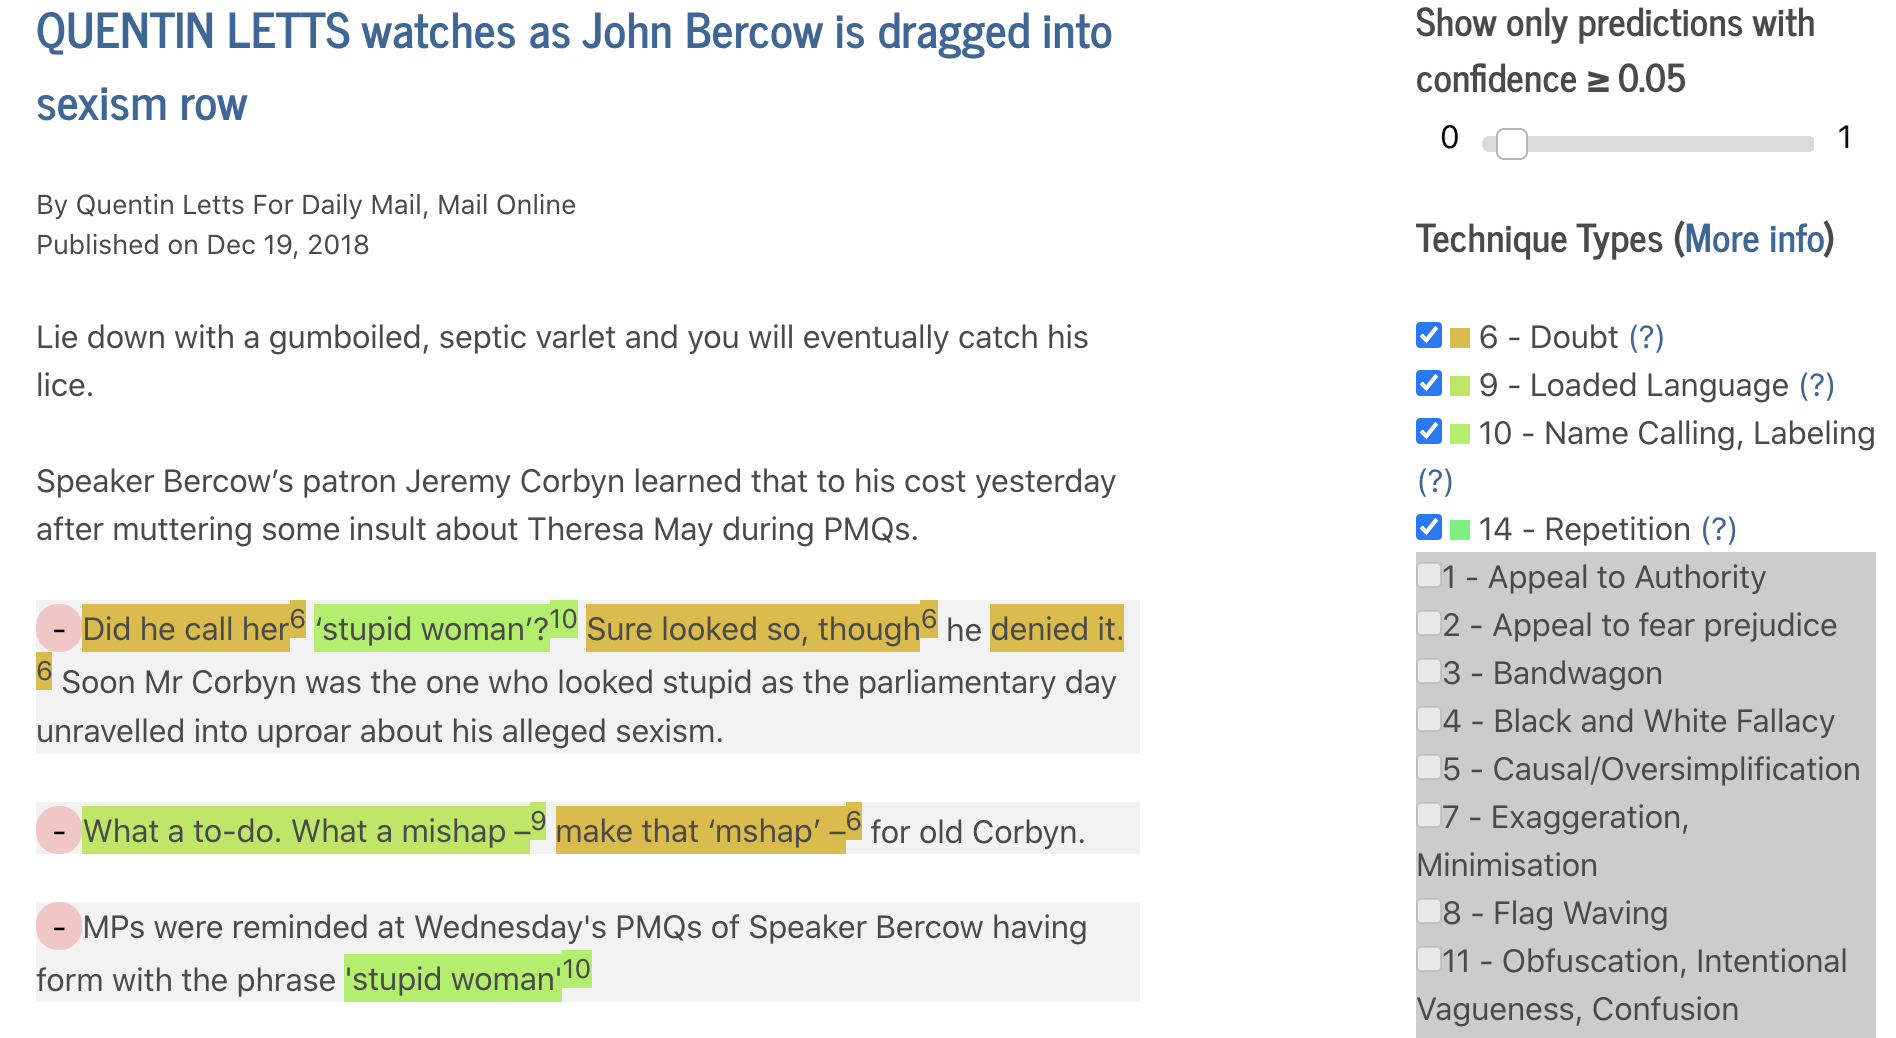
\includegraphics[width=\linewidth]{figures/brexit_propaganda.png}
    \caption{Propaganda detection on an article about a political event.}
    \label{fig:brexit_propaganda}
\end{figure}

% - Deep learning: classify spans
More recent works instead make use of complex models based on neural networks. With the advance of language models like BERT~\cite{devlin2018bert}, which are able to face different tasks with great results, more models are making use of them for almost every problem in NLP.
The work of~\citet{da2019fine}, which is focused on propaganda techniques detection, makes use of a model based on BERT.
The architecture first uses this language model to provide contextualised representations of the words, and then uses these representation to classify each word with one of the labels available (one label for each of the propaganda techniques, plus one extra label to indicate the absence of propaganda).
In this way their model needs to train only the weights of the added layer for the specific task, and reuses the rich encoded knowledge of the language owned by BERT.
In Figure~\ref{fig:brexit_propaganda}, we can see the propaganda analysis performed by this tool, which evidences the usage of several of these techniques.\footnote{\url{https://www.tanbih.org/propaganda/223/BREXIT/}}

The methods described focus on detecting how framing looks like, by highlighting occurrences which are quite visible.
But, as for the human readers, also automated methods will probably benefit by comparing different articles that present the same issue.
For example, if a detail is missing, methods like the ones presented here would not be able to see the omission.
External knowledge is required.
Related research done on verification of facts is already making use of comparison with external documents~\cite{yin2008truth}.
We would like to bring a similar analysis but with a different goal: instead of chasing the truth, we want to bring together different sides of each story, and compare their use of framing. 


% resources/datasets


% Framing and Linguistic frames (both on a single doc and on multiple docs, e.g. https://journals-sagepub-com.libezproxy.open.ac.uk/doi/pdf/10.1177/1077699015606670)


% On the other hand, there is much literature on \emph{framing}, defined
% as how a certain story is presented to shape mass opinion~\cite{goffman1974frame}, the addition to the underlying facts that reflects the sociocultural context
% %(cultural, political, ...)
% and acts as an underlying force to persuade the reader.
% % Semantic frames~\cite{fillmore2006frame}
% % News Media Frames~\cite{boydstun2014tracking} developed a schema of 15 cross-cutting framing dimensions, such as economics, morality, and politics, and
% % dataset of human annotations~\cite{card2015media}
% The work by~\cite{gamson1989media} describes a set of \emph{framing packages}, made of \emph{framing devices} (e.g., word choice, metaphors, catchphrases, 
% %exemplars, depictions, descriptions, 
% use of contrast, quantification) and \emph{reasoning devices} (e.g., problem definition, cause, consequence, solution, action%, moral evaluation
% ).



% \subsection{Related concepts}\todo{merge in techniques?}
% \label{ssec:lit_framing_other}
% % framing: exchange with other dimensions

% Difference between framing and others:
% ``framing differs from subjectivity, sentiment, bias, and related constructs. Subjectivity detection may not effectively identify well-established,
% codified frames.
% Sentiment analysis focuses on assessing the valence
% (e.g., positive, neutral, or negative) of an entity’s description. Bias involves a clear, often intentional,
% preference shown in writing for one position or opinion on an issue. In contrast, there does not exist
% a one-to-one mapping between framing and opinions (Gamson and Modigliani, 1989)
% different framings are used to support the same position on an issue. [...] identifying framing requires features and techniques that
% go beyond any one of these related concepts.''~\cite{baumer2015testing}
% Some related concepts:
% - hedging: Choi et al. (2012) identify hedging in discussion of GMOs using an SVM trained on n-grams from annotated cue phrases
% - sentiment: Greene and Resnik (2009) showed how examining grammatical construction (i.e., syntax) can reveal implicit sentiment;
% - bias: Recasens et al. (2013) used edits from Wikipedia intended to enforce a neutral point of view to identify biased sentences and the terms indicative of that bias


% \cite{mandal2017overview,gao2018neural,asghar2016automatic} (catchphrases, methaphors, causality).

% Framing manifests also through the usage of loaded language, and for this reason, \textit{sentiment and subjectivity analysis} can provide further signals~\cite{liu2010sentiment}.
% Sentiment analysis for detecting not only biased news but also comments made by news readers~\cite{park2011politics}.


% In addition to these characterisations, we can add other signals derived from studies on \emph{subjectivity}.
% % and sentiment intensity.
% % https://www.niemanlab.org/2019/05/u-s-journalism-really-has-become-more-subjective-and-personal-at-least-some-of-it/ "a blurring of the line between opinion and fact."
% As found by recent research, in contemporary journalism the line between opinion and facts is blurring more and more~\cite{blake2019news}. For this reason, having signals of subjectivity on the document and paragraph-level would be very useful~\cite{liu2010sentiment}.
% %Furthermore, subjectivity is closely related to sentiment, since sentiment analysis is about finding the value of opinion while subjectivity is about distinguishing if the text is having an opinion or just reporting factual events~\cite{liu2010sentiment}.
% In this way, each article and each paragraph can be characterised with an indication of subjectivity.

% Sensationalism:
% % http://linguistics-research-digest.blogspot.com/2014/11/sensationalism-unmasked-how-to-design.html
% The climax – the part of the story with the greatest suspense – goes first, followed by the complication – a technical term for bits of narrative that say what happened. The resolution, or the ‘how it all ended’ bit concludes the list. Beginning with the climax arouses  the reader’s curiosity and makes them want to find out more about this story.



% And there exist also works that analyse the framing of the whole news source by evaluating factors like political alignment, bias, and factuality~\cite{yin2008truth}.

% \todo{link to RQ2.1}

% % Alignment of the sources
% % Micro-level:
% % - Words that evoke framing
% % - strong sentiment, loaded language, subjectivity

% Narrative structural roles
% \cite{zahid2019towards}:
% some research considers the \emph{structural role} of a sentence in the document (e.g., is it providing some background, the main event, an evaluation).
% Different structural roles have been defined in the literature, such as 
% %Different works define sets of structural roles: 
% news schema~\cite{bell1991language}, which identifies hierarchical categories (e.g., action, reaction, consequence, context, history), narrative structure~\cite{bell2005news} (e.g., abstract, orientation, evaluation, complication, resolution), or linguistic signals~\cite{zahid2019towards,marcu2000theory}. 
% %One recent study~\cite{zahid2019towards} proposed linguistic signals to be able to recognise the structural role.
% %With such characterisations, we would be able to add to the sentence-level similarity links also their role in the different articles, to understand how their structure differs.
% Such signals could be used to identify the differences between similar sentences with regards to their structural roles in the articles. 
% % And this is an important feature because time structure and story structure are usually different~\cite{bell2005news}.

\subsection{Limitations}
\label{ssec:lit_framing_limit}

To summarise here we present the limitations found in the framing literature.

On the theoretical side, different framing techniques have been defined. Some of them, in order to be seen, require external knowledge that could be provided by using external articles.
These techniques include the omission of facts that appear on other sources, or adding details that other sources did not report because of different relevance criteria.
Or also using specific language choices that other sources do differently.
For these cases, narrowing the analysis to articles in their singularity is likely to be a limiting factor (both for human reader and for automated detection).

It is very unlikely that how the news are communicated is independent from political forces and also articles that may present 100\% factual information may result in driving the opinions in a certain way.
Given that every news source has different ideological alignment, we aim at using stories from multiple sources, written by authors with different perspectives.
In this way we can use the variety of news to our advantage, revealing even more framing occurrences.

% Limitations of single-article framing analysis
% - the method can't see what is missing or added or modified
% - narrow to one article only
% - cannot have external confirmation
% - does not see different perspectives, it just shows one side labelling as "framing biased" or not. Every source has its own biases




\section{Similarity between articles}
\label{sec:lit_relationships}

% relationships: motivation
From the motivations of the previous section, here we want to expand on exploring relationships between different articles, with the objective to use multiple sources at the same time to help facing the limitations of framing analysis.
% Just analysing the framing of single articles alone provides a good set of signals that can be used to understand the framing that is in action, and this is where the current works on framing belong to. But .
% We need the second area because we want to use methods that can tell us how similar or dissimilar are news articles or sub-parts of them.


% Definition of relationship
% \todo{link better to previous introductory paragraph}
There are different possible types of relationships between news articles, such as similarity (covering the same information), referencing (one article is citing another one), and temporal proximity. They can be performed at the document level (e.g., the whole article is similar to another one) or at the sentence level (e.g., the same sentence is corroborated by a sentence in another article~\cite{bountouridis2018explaining}) or even at the paragraph level.
Since we are interested in finding articles discussing the same information, we focus on similarity relationships.
% Other relationships could add interesting features, such as the order of publication which would help to identify which of the articles might have taken inspiration from the other. For the time being, we focus on studying and understanding the role of similarity.

% Here in this section, we first describe approaches that deal with language representation, then moving to clustering methods and then finally approaches to plagiarism detection and analysis of how the information repeats in multiple documents.
Here in this section, we first explore what we mean with similarity, then we look at how it is used, and how it is computed, concluding with some limitations of this branch of studies.
Our overall goal is to find the tools that would allow us to enrich the framing analysis by bringing information from other articles. And the articles need to relate to the same events.

\subsection{Similarity definition}
% What is similarity?

The concept of similarity is widely defined as ``\emph{the fact that people or things look or are the same}''\footnote{\url{https://dictionary.cambridge.org/dictionary/english/similarity}}. In our case, we want to focus on the specific \textbf{semantic textual similarity}, that expresses how two different pieces of text are similar considering their semantics.
This narrower definition is used in the NLP community, and for several years a specific SentEval task has been targeted to evaluate the capacity of evaluating the level of similarity between sentences~\cite{conneau-kiela-2018-senteval}.\footnote{\url{http://nlpprogress.com/english/semantic\_textual\_similarity.html}}
% exists even a benchmark that evaluates and scores the models capacity of distinguish different levels of semantic similarity between texts.
% different linguistic surface
The similarity can match with how similar the corresponding strings of the text are (character-wise similarity) but has also to account for entities, relationships and concepts that can be expressed by using different words that have the same meaning.
For example if we consider two synonyms, their semantic similarity needs to be high. 
% also dependent on the context
And another requirement is that the similarity depends on the context of the words~\cite{miller1991contextual}. The same word can have different meanings depending on the sentence it is used in.
% TODO example
% \todo{from here on, rewrite 2.2}

\subsection{Applications of similarity}
% What is similarity used for?

Similarity is used in many NLP applications that deal with documents and need to find how close they are to each others. This includes both application that work on whole documents, like document clustering, and analysis of overlap of more detailed contents that aims at finding pieces occurring in multiple documents.

% Clustering
Document clustering is widely used in the Information Retrieval community, to discover topics on different levels, to find similar items and to find possible duplicates. Given big quantities of articles, there are different methods that are able to form groups based on wider or narrower topics.

The literature is quite rich in approaches to news clustering~\cite{carpineto2009survey,jones1972statistical} %also andrews2007recent
that work in many different ways.
Some clustering techniques requires specifying the number of clusters wanted (K-Means, Mean-Shift, GMM) as an input, others instead are more flexible, discovering the number of cluster based on other geometric properties (DBSCAN).
And some others have even nicer properties.
For example, Agglomerative Hierarchical Clustering allows cutting at different stages of the algorithm which represent a threshold distance to merge clusters.


% clustering techniques to find similarity relationships both at the article level (to identify articles that talk about the same event) and at the sentence level (to identify parts of article, details, which are similar, in order to be able to relate sub-document parts).




% Plagiarism and Manipulation detection (diff\&co)
Then there are applications of similarity at a more fine-grained level.
The overall objective of this group of works is to study how many parts of a document also appear in other documents.
% - plagiarism
The objectives for this analysis may vary from plagiarism detection~\cite{potthast2010evaluation} where the occurrence of text pieces too similar is an indication of non-originality.
% - finding external confirmation in fact-checking
Or in the fact-checking perspectives, when external confirmation is searched about a specific detail to be able to corroborate and establish if the content is true~\cite{TODO}
% - bountouridis
Or to compute how complete is the reporting from different sources, analysing the overlap between different articles.

% % TODO figure sent-sent similarity
% Some methods are able to extract which information appears in multiple documents or is omitted in some others~\cite{bountouridis2018explaining}, being really useful to analyse the selection of details that each article has made.

% % why
% Once the articles and parts of them are linked in clusters, there are some works that exploit this information to see how much information is shared between them.
% This is the field of plagiarism detection, or also some other works that compute how much information is corroborated externally or omitted.


% Corroboration analysis
% % what (details)
% Furthermore, there are works that not only link the articles at a document level, but also investigate in more detail the connections between sentences.
In one recent work~\cite{bountouridis2018explaining}, groups of similar articles are found, then broken down to pieces of information and analysed to find if these details are \emph{corroborated} (occurring in multiple documents) or \emph{omitted} (occurring in other documents of the same group, but not the current one). 
\todo{figure from Bountouridis paper?}
%is good for getting relationships between paragraphs and documents. Corroboration and omission
% \begin{added}
We aim to use this idea of applying similarity to both article-level and sentence-level, extending it even to the word-level. By doing so,
not only we might be able to recognise which sentences appear in multiple documents (with different degrees of similarity) but also we would be able to identify the specific words that have been changed.




% Even for recommender systems (user-items recommendations based on similarity)

\subsection{Similarity computation}
% How is similarity computed?
In order to be able to compute a similarity between different texts, there are two steps: \emph{i)} representing the texts with a numeric representation, \textit{ii)} use similarity metrics between these representations.

% Language representation
The first step is the one that is more interesting and so many different methods exist.
% why
The aim of group of methods is to find a condensed representation that contains the meaning of the text, independently from its length.
% \emph{What is contained in the text?}

% what (details)
Starting with very naive methods, we have approaches based on \emph{bag of words} that simply take into consideration which words are present in the considered text.
They run with an initial scan of all the available documents to create a dictionary, and then each document is represented with a one-hot-vector that is saying for each word in the dictionary if it belongs to the current document.
Many refinements to this basic approach exist, e.g., by removing words that do not carry meaning (stopwords) or by limiting the dictionary based on term frequencies (only the top k words overall are considered, or only words that appear at least n times).
This group of methods culminates with a model that is called TF-IDF~\cite{ramos2003using} which is based on two components: Term Frequency and Inverse Document Frequency.
In simple words, the first component gives higher weights to terms that appear more in the considered document, while the second measures how important a term is by promoting rare terms~\cite{jones1972statistical}.

Then we have another group of models that relies on explicit semantic representation. This is the field of knowledge extraction that is based on recognising the entities mentioned in a text (entity recognition and linking) and extracting the relationships expressed between them. Using these models, a text is translated into a knowledge graph.
The main limitations of this set of models it that they may work accurately enough just when entities that are known are mentioned, and need to be supervisioned with rich knowledge bases.

And finally, we have a whole line of research that is based on distributional semantics.
The assumption is that the words take their meaning from the context around them. For example two synonyms can be recognised as similar because one can be switched for the other and therefore they have similar contexts.
This unsupervised learning strategy therefore builds words representation by observing their context.
A milestone in this area is given by the word embedding models Word2Vec~\cite{TODO} and GloVe~\cite{TODO} which have shown their superiority in a big variety of tasks.
They are able to work with syntax and semantics and even solve analogy tests~\cite{mikolov2013efficient} with great performances.

Then in the recent years, new models have arisen in the language representation that are extremely powerful to encode entire documents and capture their meaning. It is the
era of
% Language Models~\cite{devlin2018bert,cer2018universal,yang2019xlnet}.
% With the recent explosion of Deep Learning representation there emerged many of
Language Model that can provide document representation, like BERT~\cite{devlin2018bert}, XLnet~\cite{yang2019xlnet}, or even more oriented towards the similarity task: Universal Sentence Encoder~\cite{cer2018universal}.
And all these models can be used directly without the need to be trained, thanks to pre-trained models that perform already well out-of-the-box.

% strenghts, limitations
The main strength of Language models is that they are able to
relate documents that talk about the same events, even if they use different linguistic surface, from articles that may use the same subset of words but talk about different events.
It is a semantic matching more than a word-based matching which accounts for the specific order of words (problem of previous models). 
The semantics they are able to express
is shallower with respect to the explicit semantics based on Entity Linking, but it is more resistant to changes in the linguistic surface and works without having knowledge bases encoding the reality.

% Talk about SentEval\footnote{\url{http://nlpprogress.com/english/semantic_textual_similarity.html}}: benchmark that evaluates the ability of models to score similarity of sentences


% % language representation
% And with the recent advance of language models~\cite{devlin2018bert,cer2018universal,yang2019xlnet}, we have available robust methods to analyse the overlap of different articles and sub-parts of them by using their representation.







% Specific similarity functions: euclidean, cosine, ...
Once these models synthesise documents of different length into numeric representations, there are different geometrical measures that can be used to compute the distance or similarity.
The most commonly used distance measure is Euclidean, although with word and sentence embedding usually the cosine similarity is more common.

And we can compare therefore representations for single words, for sentences or even for complete documents.
The computation of similarity allows to target all the different applications that we saw previously, exploring commonalities and differences at multiple granularity levels.
\todo{a figure of sentence comparison to show this?}


% Example: let us compare TF-IDF, BERT and USE matrices (similar to experiment)
% \todo{finish, link to the discourse}



% \subsubsection{News Clustering}
% Clustering

% % why
% Once documents and sentences are transformed to a representation, we can apply clustering techniques to find similarity relationships both at the article level (to identify articles that talk about the same event) and at the sentence level (to identify parts of article, details, which are similar, in order to be able to relate sub-document parts).

% % what (details)
% LDA
% methods mostly used are Latent Dirichlet Allocation (LDA) or document embedding.
% % News aggregators and LDA topic: can provide article-level aggregation
% LDA~\cite{blei2003latent} is the most used technique for topic modelling, as it allows the discovery of topics and to group articles accordingly using word distributions.

% Cliques

% Distance-based

% Hierarchical Clustering

% % Topic Detection and Tracking steps
% % 0. flat clusters: TDT before 2003. Simple LDA clustering methods
% % 1. hierarchical topics: TDT 2003 (hierarchy of topic --> event --> story)
% % 2. dependencies: 2004 Napallati~\cite{nallapati2004event}. They introduce edges with two possible reasons: causality or only temporal ordering.

% % News event structure evolution (keep short)
% % Instead in the direction of the structure of news event, we have a succession of works that went more in details than just creating groups / flat clusters generated by LDA.
% % First of all \emph{hierarchical} topic modelling~\cite{allan2003flexible} that defined a set of levels (from the broad concept of topic, to the narrow event that belongs to the topic, and then a specific story/anecdote).
% % And then moved to study the dependencies between events~\cite{nallapati2004event} with causality and temporal ordering.
% % This recently brought to approaches that are able to find the events belonging to a topic and link them creating a Event Evolution Graph~\cite{yang2009discovering,ansah2019graph} that can be visualised to give an idea of the dependency between the events detected.
% %\todo[color=yellow]{The removed paragraph was about events hierarchy and dependency}
% % ~\cite{ansah2019graph} that is able to generate a visual story timeline summarisation, connecting the main events; Event Maps~\cite{yang2009discovering}
% % Or works that focus on the illustrative side and use the extracted story timeline summarisation~\cite{ansah2019graph}.

% % Furthermore, \cite{cai2019temporal} also presents event maps (original baseline~\cite{yang2009discovering}). With also importance score on the nodes and edges. The event relationships can be temporal, content dependence and event dependence.



% % strengths, limitations


% The literature is quite rich in approaches to news clustering~\cite{carpineto2009survey,jones1972statistical} %also andrews2007recent
% that can bring together articles talking about the same events.










% \subsubsection{Corroboration analysis}
% Corroboration analysis

% % what (details)
% Furthermore, there are works that not only link the articles at a document level, but also investigate in more detail the connections between sentences.
% In one recent work~\cite{bountouridis2018explaining}, groups of similar articles are found, then broken down to pieces of information and analysed to find if these details are \emph{corroborated} (occurring in multiple documents) or \emph{omitted} (occurring in other documents of the same group, but not the current one). 
% \todo{figure from Bountouridis paper}
% %is good for getting relationships between paragraphs and documents. Corroboration and omission
% % \begin{added}
% We aim to use this idea of applying similarity to both article-level and sentence-level, extending it even to the word-level. By doing so,
% not only we might be able to recognise which sentences appear in multiple documents (with different degrees of similarity) but also we would be able to identify the specific words that have been changed.




% Citation Networks?

% Edit distances?

% Time evolution? TODO find stuff

\subsection{Limitations}
\label{ssec:lit_relationships_limitations}
% The main problems of this set of approaches:
% - analysis of what the differences mean is left to the reader

% strengths, limitations
However, this set of approaches is limited to bringing to the attention of the reader the linked information pieces with a measure of similarity, without characterising the differences.
The reader would then need to evaluate the impact of each of the multiple versions of the texts, and the framing that they imply. 
Different documents may express the same set of details, but give them a different role (reporting an action, commenting, contextualising, doing a digression, identifying causes and consequences) and use different words that are semantically similar but may imply a different framing perspective.
And also the fact that a certain detail is present or not in certain articles within a group where other sources mention it, needs to be analysed with framing theories.


Another limitation of this group of works is that, while they analyse the overlap of information, they do not consider the influence between the sources (one could have taken the content from the other and modified it slightly).
This problem is currently tackled by works on plagiarism analysis, but this is not studied jointly with framing analysis.
And furthermore plagiarism detection is done by having one questionable article and a set of original works, while here we do not have this distinction.
% What plagiarism analysis tells us is that two documents have highly similar parts between them.
We would like to analyse how the same information is recycled and slightly changed, by tracking it across several news sources.
% time features that could signal the direction of 
% Motivation for RQ2.2: overlap of information is high. Is it a coincidence? Or there is a flow of information / recycle between news sources? Who uses contents from the others, and how is it modified?




\section{Comparing different perspectives}
\label{sec:lit_gap}
% limitations
Although these two previous research areas have done significant progress, they have evolved independently without many points of contact.
We need to bring together the works on framing and on similarities in order to spot more subtle examples of framing.

\begin{figure}[!htb]
    \centering
    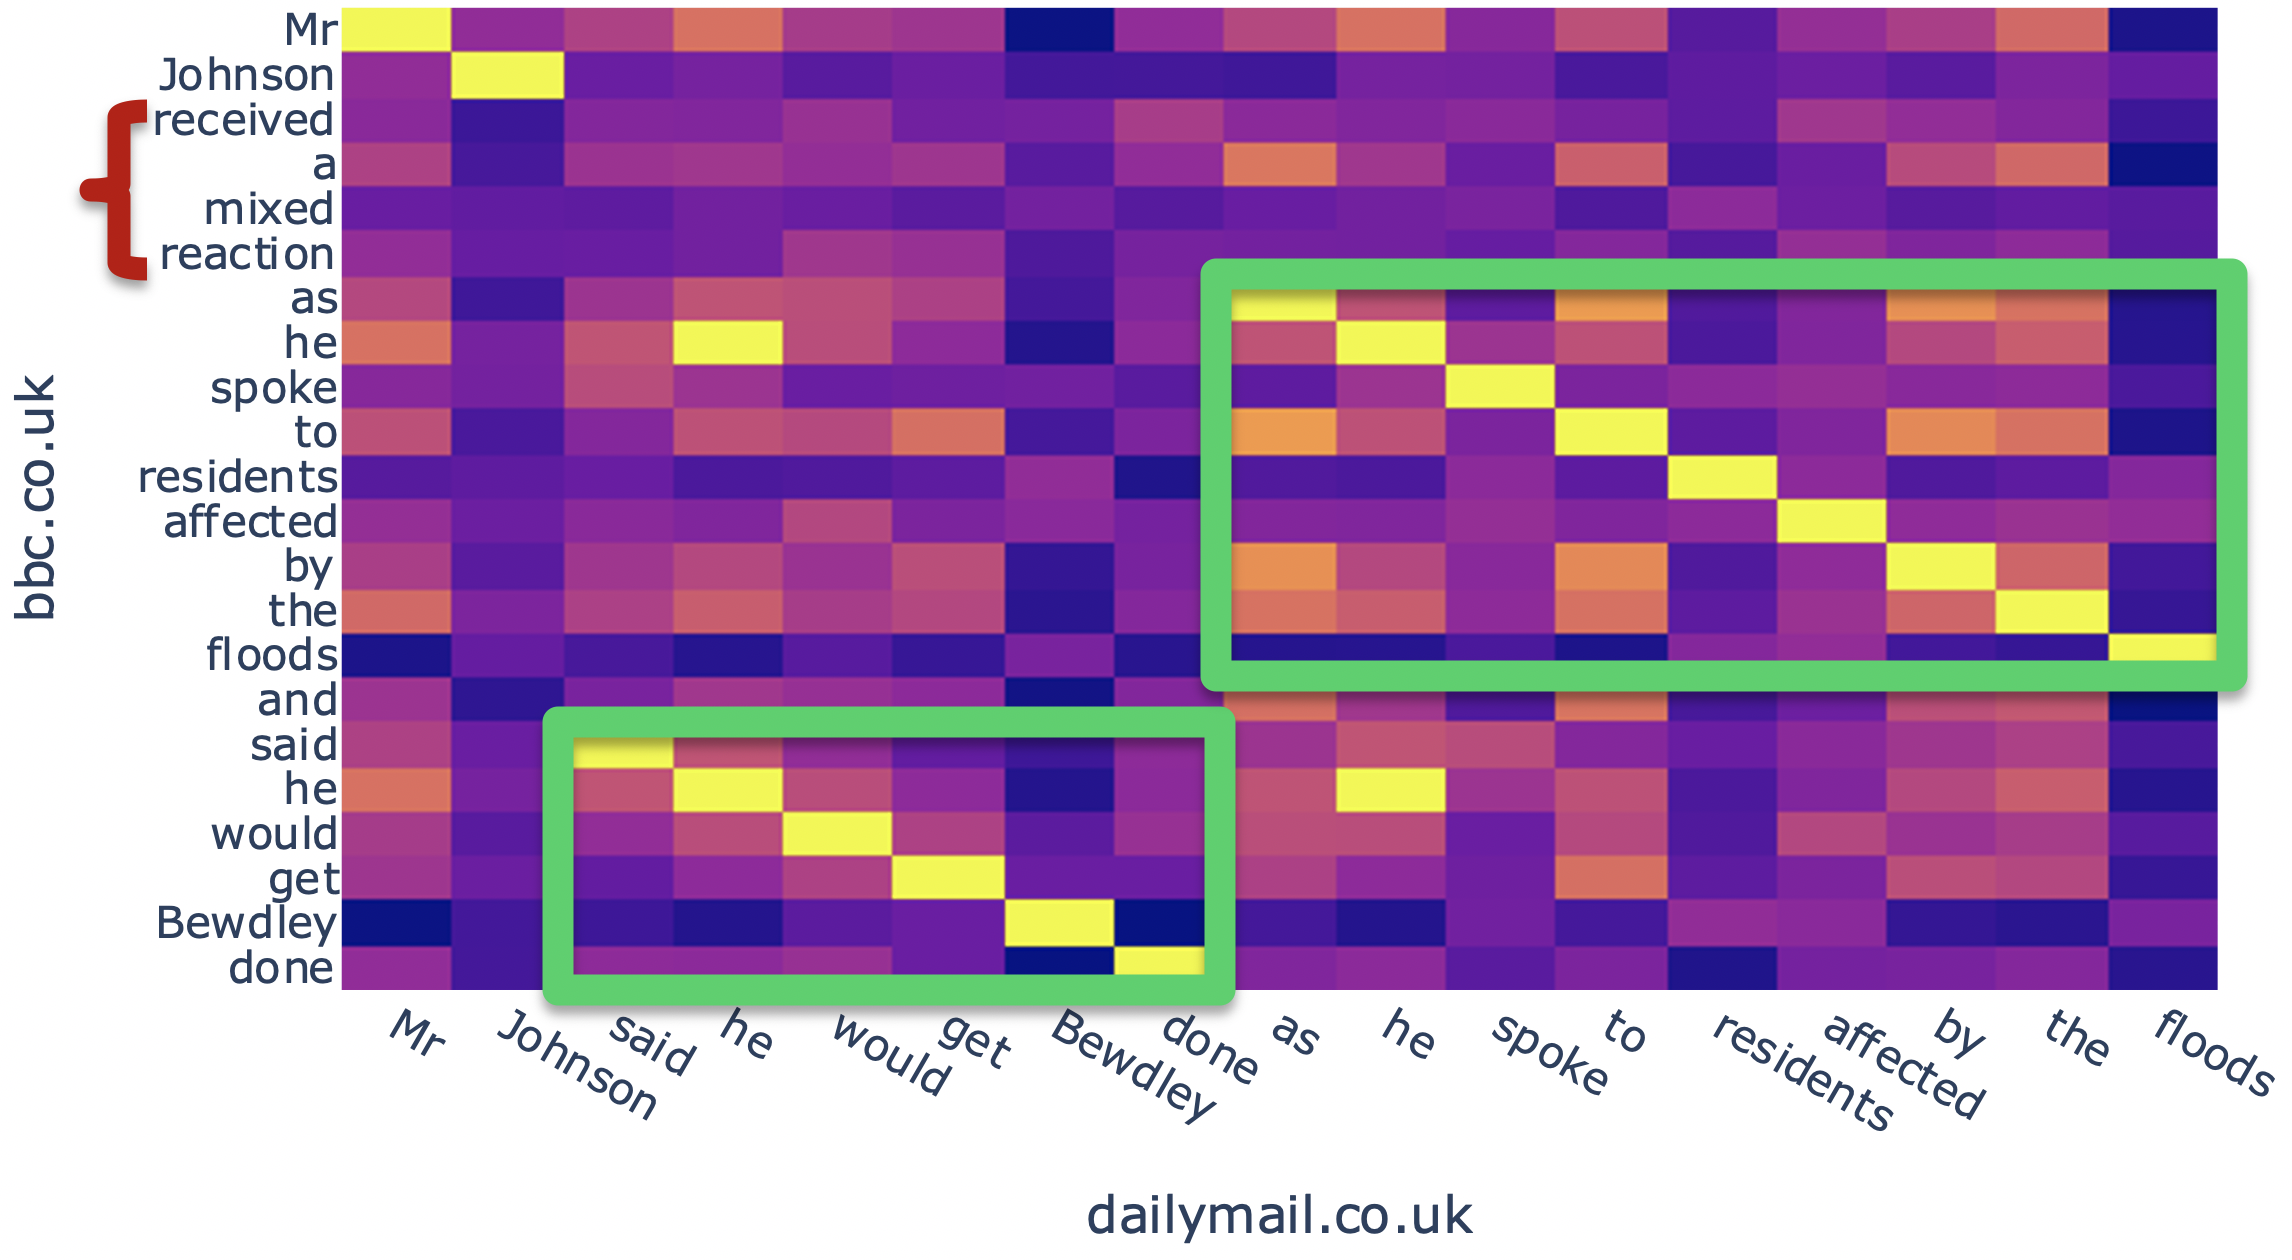
\includegraphics[width=\linewidth]{figures/johnson_flood.png}
    \caption{Example where omitting a detail provides a different framing.}
    \label{fig:johnson_flood}
\end{figure}

% example that needs cross-article analysis
If we take the example of Figure~\ref{fig:johnson_flood}, we have two sentences coming from two different news outlets (on the vertical axis from BBC\footnote{\url{https://www.bbc.co.uk/news/uk-england-hereford-worcester-51791346}} while on the horizontal from Daily Mail\footnote{\url{https://www.dailymail.co.uk/news/article-8088805/Britons-facing-heavy-downpours-four-inches-rain-50mph-winds-set-batter-UK.html}}) and compare the words they contain by using a similarity metric~\cite{cer2018universal}.
From this figure we can see that in the green boxes we have information reported from both sources, while in the red curly brace we have a detail that has been reported only by the BBC.
This specific detail, describing a ``mixed reaction'', gets omitted from the sentence from Daily Mail that is known to be right-leaning.\footnote{\url{https://mediabiasfactcheck.com/daily-mail/}}
% Daily Mail: "While many locals greeted him warmly, he also faced heckles of 'traitor' as he viewed flood barriers - and one person told him to 'do your f***ing job' as he posed with teenagers for a selfie on a bridge in the town."

% limitation of current framing
This example present one specific manifestation of framing that current techniques do not focus on detecting, that is the selection of details.
And the main reason is that such techniques requires a method that goes beyond the analysis of one single article at a time.
We cannot know when something has been omitted if we don't have or a ground truth or different stories to corroborate with, using the richness of information available from multiple points of view.
% RQ1.1 lift
There are facets of framing that have not been tackled by automated approaches because they cannot be pointed out by considering a single article, and we need to investigate which ones we can define more rigorously and how important they are.

% acknowledge existing works on framing differences, but manual and not annotated
% Manual framing difference approaches
There exist some efforts in this joint area, that try to provide multiple points of view of the same events by considering sources that come from different political leanings.
For example, AllSides\footnote{\url{https://www.allsides.com/story/admin}} is a platform that collects articles from different news sources providing a hand-curated set of stories where articles with different political bias are put together, with also a brief textual introduction of the framing differences.

\begin{figure}[!htb]
    \centering
    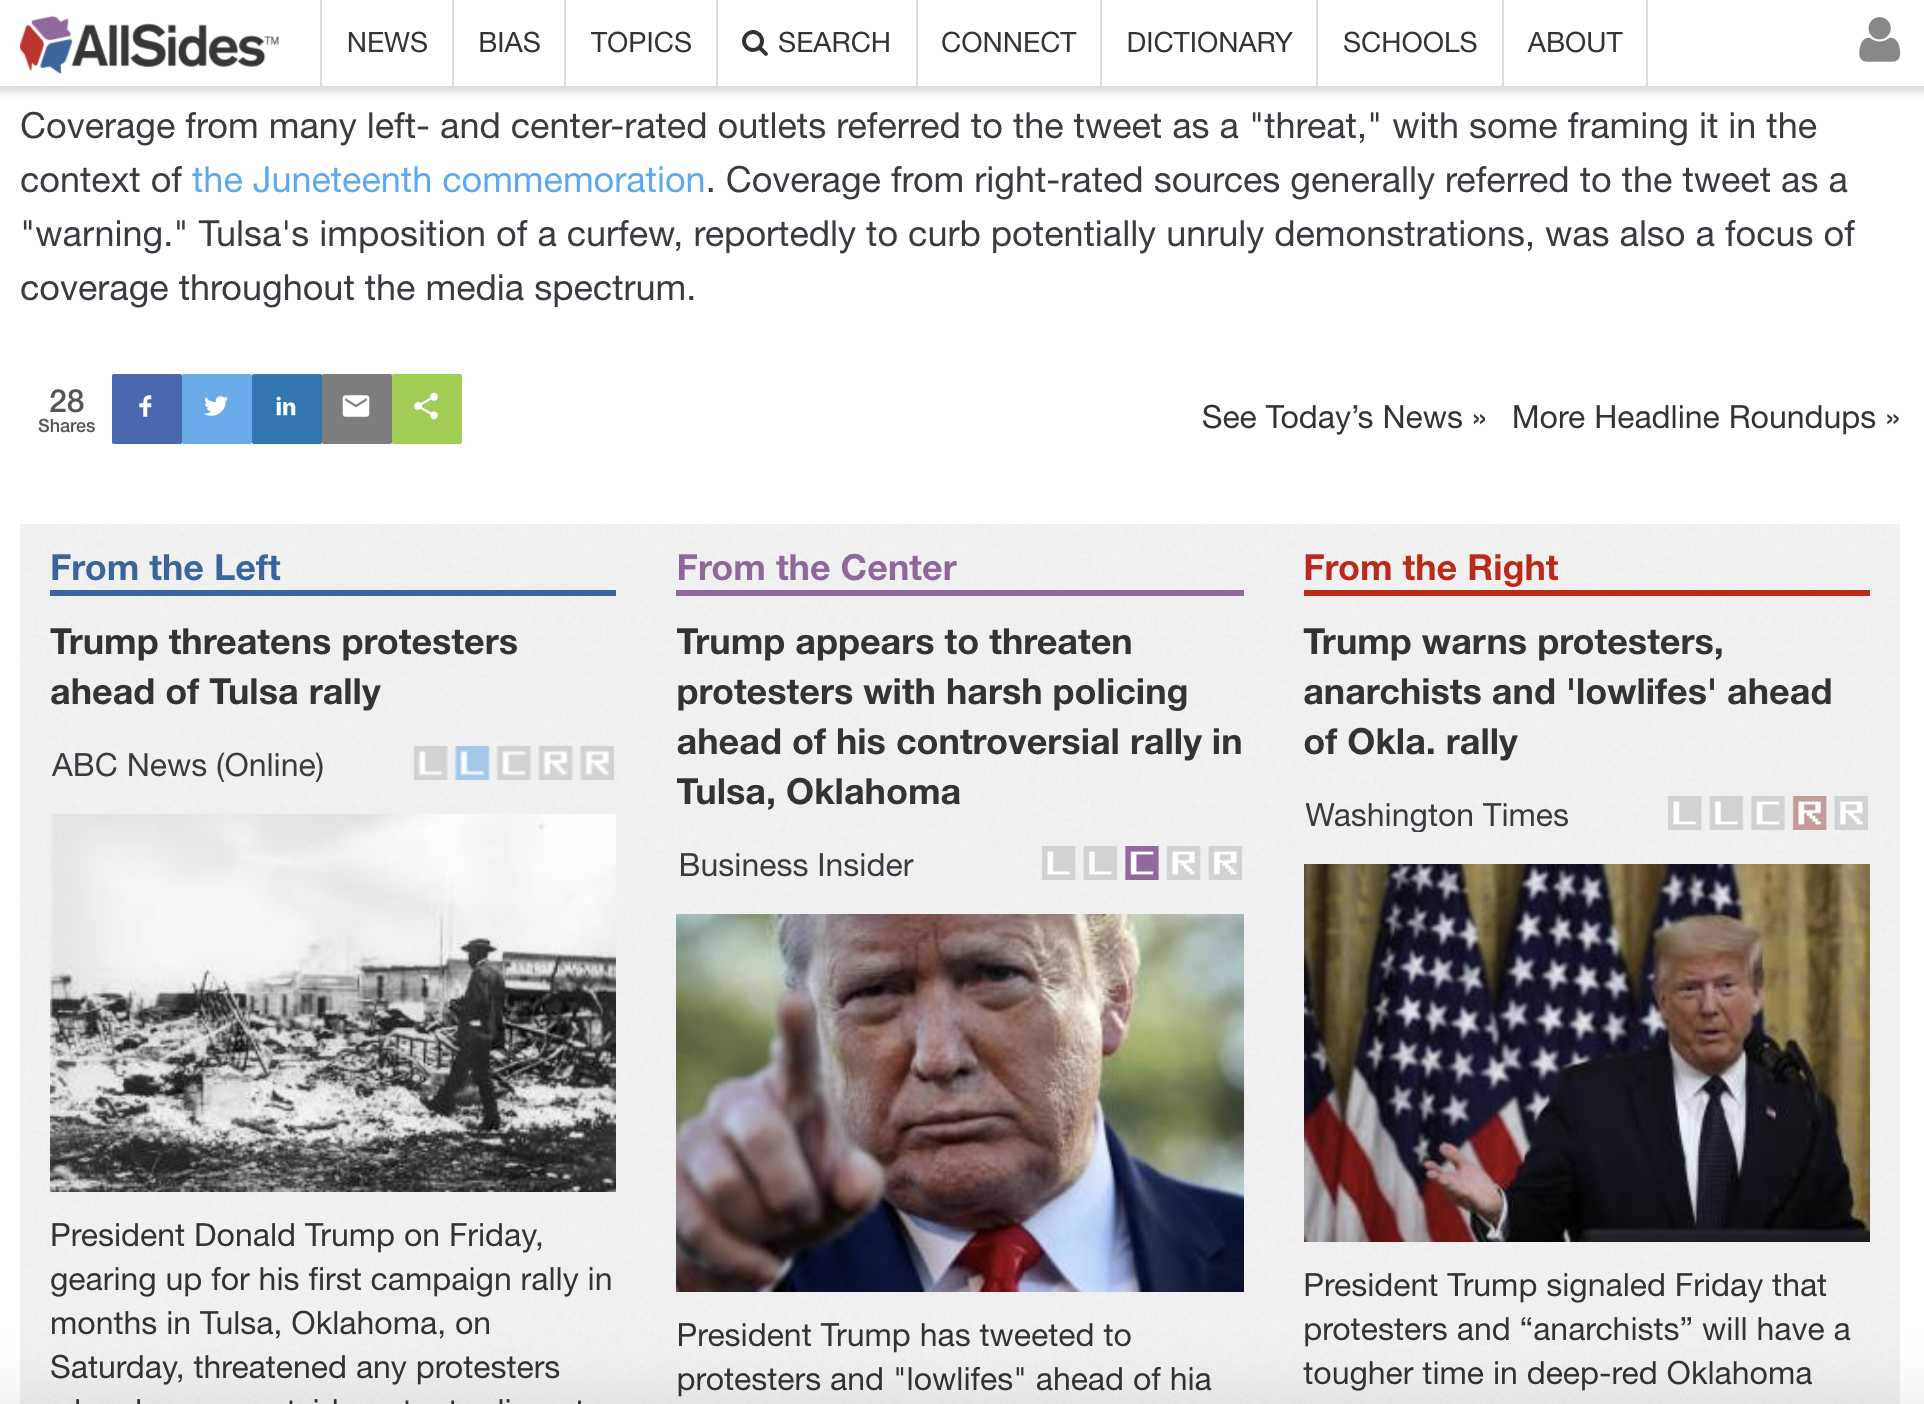
\includegraphics[width=\linewidth]{figures/allsides.png}
    \caption{Example of analysis from AllSides: \url{https://www.allsides.com/story/trump-tweets-about-protesters-ahead-saturday-tulsa-rally}}
    \label{fig:allsides}
\end{figure}

In Figure~\ref{fig:allsides} we can see an example that is displaying how a source from the left, one from the center and one from the right frame differently Trump tweeting about his upcoming rally in Tulsa.
% - which signals
Sources from the left use the term ``threat'' while sources from the right use ``warning'', which can be seen in the specific words used in the headlines.
This \emph{selection of terms} gives a specific framing which can be seen as an emphasis from the left on the strength of the tweet versus an attenuation from the right, plus the centre is instead keeping in an intermediate position.
But if we look at the articles, this term is not the only difference. The sources from the left give more space to the narrative about Juneteenth\footnote{\url{https://en.wikipedia.org/wiki/Juneteenth}} and the past history of the city, which emerges also in the image of the article from ABC News.
We need to have a more precise definition of what constitutes framing and how it manifests in the articles.
% - how could we detect
% - bias vs framing?
% \todo{say that framing/propaganda detection is not able to pick up these differences}

% limitations:
% Only US, handmade (lift RQ1.2)
Considering AllSides, its main limitations are due to the fact that the analysis is handmade and therefore they publish just a few stories per week and only focusing on the US.
With this work we want to provide a similar analysis but powered by an automated method, which will need to rely on existing works of framing analysis and document similarities.

% \todo{limits of automated framing / propaganda analysis: https://propaganda.qcri.org/}


% - break your bubble and similar (Blue Feed, Red Feed): feed populated with news from different sides. But not specific on a certain event.

% lack of automated framing difference analysis
We argue that by the integration of these two fields, a deeper analysis of framing can be achieved, with the goal to understand better how, from the same event, multiple stories are generated.

% Framing analysis, being limited to single-article analysis, cannot analyse specific framing manifestations that have been described in theoretical works: for example selecting or omitting details. This is the area that we want to tackle.

% just left-right political leaning is considered (lift RQ2.1)
With respect to AllSides or other tools (Blue Feed, Red Feed\footnote{\url{https://graphics.wsj.com/blue-feed-red-feed/}}) that just focus on the left/right political bias (mainly from US with liberal/conservative), we want to conduct an analysis that compares several characteristics of the news outlets, such as the newsgroup they belong to, or how they are rated by multiple news rating organisations (factuality, bias), or their ideology in general.
We want to have an idea of the correlation between certain features of the sources and the type of framing that they use. This goes beyond the left/right spectrum because not all the news is focused on the political topic.


% lift RQ2.2
Furthermore, seeing that the overlap of information between the different sources is quite high, we want to analyse more deeply how the content is reused by different sources (as evidenced in \ref{ssec:lit_relationships_limitations}). The main focus is not in evidencing plagiarism (as other studies have done), but instead to find how the news is modified considering the time of publishing.
% Motivation for RQ2.2: overlap of information is high. Is it a coincidence? Or there is a flow of information / recycle between news sources? 
We need to investigate which sources use contents from others, and how they slightly modify the information contained to provide a different perspective.

% 1.1 Need for cross-article signals

% 1.2 Need for baseline

% 2.1 Correlation source bias/features

% 2.2 Temporal chains





% \section{Early draft - remove and merge}

% For this reason, in this chapter we first focus on works that analyse how documents are talking about the same details, using language representations, clustering and seeing which details are narrated by different sources.
% The objective of this first group is to extract the common ground between different stories and highlight the pieces that are uniquely changed, added or removed by individual sources.

% Then we present works that characterise documents with linguistic features that we aim to use for the second phase, that is \emph{understanding} the framing that the choices of the authors use. For this reason, we analyse a set of features that have appeared in similar works.





% \section{Linguistic features}

% While the first group of works focuses on finding similar articles and highlighting parts that are similar or different, here we present a set of linguistic features that can be very useful in order to characterise the peculiarities. These works are usually independent from our goal, and are applied in a wide variety of tasks.

% \subsection{Natural Language Parsing}

% % grammar, POS, dependencies, entity extraction and linking
% First of all, we have a set of features that comes to represent the structure of sentences. It is the world of parsers, that are able to tokenise, find Part Of Speech and create Dependency Trees.

% The progress of this research is quite advanced, and there are plenties of tools available off-the-shelf (e.g. Stanford NLP, SpaCy, ...) that achieve good performances (TODO?)

% entities (WARNING: avoid duplicate with 2.1.1. Language Representation)



% \subsection{Bias and Framing}



% \section{Gaps}

% TODO: underline lack of approaches and studies that accomplish the task automatically.

% All these features have been used in previous research, but as mentioned above, they are mainly applied to single-article analysis. Extending this kind of analysis by taking into consideration the relationships both at the article level and the sentence level would bring a big contribution by providing contrastive signals that would not come up otherwise. 

% \label{sec:related}

In this section, we provide an overview of previous studies in two areas of research. First, the investigation on relationships between news articles which aims to find documents that cover the same information. Second, the detection of narrative linguistic signals, which investigates and characterises several aspects of structure, framing, and subjectivity.
For both of them, we gather a set of techniques that enable our approach described in the next Section~\ref{sec:framework}.
%can be used to characterise the components(sentences/paragraphs) of the articles.
%can help us characterise the narrative comparison analysis.
%Starting from approaches that link together articles and parts of articles together that cover the same information, we see how we can enrich and characterise the participating nodes (articles and sentences) with signals from narrative, framing and subjectivity analysis.

%\todo[color=yellow]{add a sentence here to remark that we just observed works on the two areas, separated and not joint?}

\begin{comment}
    % 2: Main limitations of existing works
    But there are different limitations of what is available.
    For example, the approach proposed by~\cite{bountouridis2018explaining} finds and links similar articles and similar sentences (POI) in them, but mainly focuses on finding indications of corroborated information or omitted information.
    Their work does not investigate the differences between the linked pieces, accounting for subtle modifications and their exploitation to provide bias / subjectivity (framing / word choices).
    Another recent work~\cite{zahid2019towards} instead is just focusing on a single article narrative analysis, without linking and comparing it to other news articles.
    \todo[color=yellow]{move this paragraph to related work, just leave a sentence here}
\end{comment}

\subsection{Relationships between news articles}

% Definition of relationship
There are different possible types of relationships between news articles, such as similarity (covering the same information), referencing (one is citing another one), and temporal proximity. They can be performed at the document level (e.g., the whole article is similar to another one) or at the sentence level (e.g., the same sentence is corroborated by a sentence in another article~\cite{bountouridis2018explaining}) or even at the paragraph level.
Since we are interested in finding articles discussing the same information, we focus on similarity relationships.
% \begin{added}
Other relationships could add interesting features, such as the order of publication which would help to identify which of the articles might have taken inspiration from the other. For the time being, we focus on studying and understanding the role of similarity.
% \end{added}
%In this direction it is very important to keep exposed to multiple perspectives~\cite{flaxman2016filter}, thanks to news aggregators, that provide articles on the same events from multiple sources (e.g. Google Headlines\footnote{\url{https://news.google.com/}}) or approaches that analyse the corroboration and omission between news articles~\cite{bountouridis2018explaining}. 

% Article-level relationships
At the article-level, there is a wide variety of work that investigates article clustering, and the methods mostly used are Latent Dirichlet Allocation (LDA) or document embedding.
% News aggregators and LDA topic: can provide article-level aggregation
LDA~\cite{blei2003latent} is the most used technique for topic modelling, as it allows the discovery of topics and to group articles accordingly using word distributions.
% similarity measures
Another technique for grouping articles together is to compute a similarity measure (e.g., cosine similarity) between numeric representations of the documents (TF-IDF~\cite{jones1972statistical} or Language Models~\cite{devlin2018bert,cer2018universal,yang2019xlnet}).
% \begin{added}
We plan to study these models in order to select the one that can efficiently discriminate articles that talk about the same events, even if they use different linguistics, from articles that may use the same subset of words but talk about different events. 
% \end{added}
%In this direction, there are several techniques, such as TF-IDF~\cite{jones1972statistical} or using representations coming from Language Models~\cite{devlin2018bert,cer2018universal,yang2019xlnet}.
% recent advances on similarity and document embedding
%But with the recent explosion of Deep Learning representation there emerged many of Language Model tools that can provide document representation, like BERT~\cite{TODO}, XLnet~\cite{TODO}, or even more oriented towards the similarity task: Universal Sentence Encoder~\cite{TODO}.\todo[color=yellow]{too many details on possible features for similarity?}
% And all these models can be used directly without the need to train, thanks to pretrained models that perform already well out-of-the-box.


% Topic Detection and Tracking steps
% 0. flat clusters: TDT before 2003. Simple LDA clustering methods
% 1. hierarchical topics: TDT 2003 (hierarchy of topic --> event --> story)
% 2. dependencies: 2004 Napallati~\cite{nallapati2004event}. They introduce edges with two possible reasons: causality or only temporal ordering.

% News event structure evolution (keep short)
% Instead in the direction of the structure of news event, we have a succession of works that went more in details than just creating groups / flat clusters generated by LDA.
% First of all \emph{hierarchical} topic modelling~\cite{allan2003flexible} that defined a set of levels (from the broad concept of topic, to the narrow event that belongs to the topic, and then a specific story/anecdote).
% And then moved to study the dependencies between events~\cite{nallapati2004event} with causality and temporal ordering.
% This recently brought to approaches that are able to find the events belonging to a topic and link them creating a Event Evolution Graph~\cite{yang2009discovering,ansah2019graph} that can be visualised to give an idea of the dependency between the events detected.
%\todo[color=yellow]{The removed paragraph was about events hierarchy and dependency}
% ~\cite{ansah2019graph} that is able to generate a visual story timeline summarisation, connecting the main events; Event Maps~\cite{yang2009discovering}
% Or works that focus on the illustrative side and use the extracted story timeline summarisation~\cite{ansah2019graph}.

% Furthermore, \cite{cai2019temporal} also presents event maps (original baseline~\cite{yang2009discovering}). With also importance score on the nodes and edges. The event relationships can be temporal, content dependence and event dependence.


% Corroboration, external confirmation / denial: computation and visualisation. \cite{bountouridis2018explaining}
Furthermore, there are works that not only link the articles at a document level, but also investigate in more detail the connections between sentences.
In one recent work~\cite{bountouridis2018explaining}, groups of similar articles are found, then broken down to pieces of information and analysed to find if these details are \emph{corroborated} (occurring in multiple documents) or \emph{omitted} (occurring in other documents of the same group, but not the current one). 
%is good for getting relationships between paragraphs and documents. Corroboration and omission
% \begin{added}
We aim to use this idea of applying similarity to both article-level and sentence-level, extending it even to the word-level. By doing so,
not only we might be able to recognise which sentences appear in multiple documents (with different degrees of similarity) but also we would be able to identify the specific words that have been changed.
%, on one side we will be able to keep the information of similarity and on the other side we will bring into view the differences of the articles (sentences) and sentences (words).
% \end{added}

% \removed{When looking at the results of such approaches, it is often left to the reader to evaluate and compare the linked information pieces.}
% \begin{added}
However, this set of approaches are limited to bringing to the attention of the reader the linked information pieces with a measure of similarity, without characterising the differences. The reader would then need to evaluate the differences in the role of the sentence, the framing that it implies and how it compares with other sentences in terms of subjectivity.
Different documents may express the same set of details, but give them a different role (reporting an action, commenting, contextualising, doing a digression, identifying causes and consequences) and use different words that are semantically similar but may imply a different framing perspective.
For this reason, the next subsection presents a set of narrative linguistic signals that could provide us with the missing features.
% \end{added}
% \removed{A sentence can have different roles in a document (reporting an action, commenting, contextualising, doing a digression) and hence it is important to extract and present these features.
% Furthermore, even if the information is reported in similar ways in different articles, they could be using specific choices of words to provide a different framing.}
%We see these difference, as signals, in the following subsection.

%The only cross-document narrative analysis found~\cite{reiter2014nlp} (structural similarity, using FrameNet)~\todo[color=yellow]{move this sentence in the proper position}

% Some directions used by document comparison:
% - fact-checking: \cite{karadzhov2017fully} automatic fact-checking by comparing news article
% - perspectrum: \cite{chen2019seeing} presents PERSPECTRUM, comparing stance and perspectives for a claim.
% - break your bubble or similar news aggregators (Balancer, Blue Feed Red Feed, Burst your bubble, Escape your bubble, Read Across the Isle, OneSub, Nuzzera)

\subsection{Narrative linguistic signals}
% \subsection{The many faces of \sout{biases}: Narrative, framing and subjectivity/bias signals}
%\todo{define somewhere the term \emph{narrative linguistic signal}}
% The term mainly comes from http://ceur-ws.org/Vol-2342/paper9.pdf where they use "linguistic devices". "Devices" was then substituted with "signals". About "linguistic signal", there are many works that use it https://www.aaai.org/ocs/index.php/ICWSM/ICWSM16/paper/download/13112/12731 https://www.shanjiang.me/publications/cscw18a_paper.pdf
% It's in general some words that signal something (structure / framing / subjectivity). And "narrative" because it encloses structure, framing and subjectivity. 

There is much research on exposing the narrative using linguistic signals~\cite{zahid2019towards}, with specific words that indicate the \emph{structural role}, \emph{framing} and \emph{subjectivity} of the part of text they belong to.
%There is a wide literature of work that wants to expose the narrative using linguistic signals, with specific words that indicate the \emph{structural role}, \emph{framing} and \emph{subjectivity} of the part of text they belong to.
One limitation is that most of such works are applied to single articles, with little comparison between them.
%\todo[color=yellow]{put this at the end of subsection, to bridge what we want to do?}

% news schema structure
On one hand, some research considers the \emph{structural role} of a sentence in the document (e.g., is it providing some background, the main event, an evaluation).
Different structural roles have been defined in the literature, such as 
%Different works define sets of structural roles: 
news schema~\cite{bell1991language}, which identifies hierarchical categories (e.g., action, reaction, consequence, context, history), narrative structure~\cite{bell2005news} (e.g., abstract, orientation, evaluation, complication, resolution), or linguistic signals~\cite{zahid2019towards,marcu2000theory}. 
%One recent study~\cite{zahid2019towards} proposed linguistic signals to be able to recognise the structural role.
%With such characterisations, we would be able to add to the sentence-level similarity links also their role in the different articles, to understand how their structure differs.
Such signals could be used to identify the differences between similar sentences with regards to their structural roles in the articles. 
% And this is an important feature because time structure and story structure are usually different~\cite{bell2005news}.

% framing
On the other hand, there is much literature on \emph{framing}, defined
as how a certain story is presented to shape mass opinion~\cite{goffman1974frame}, the addition to the underlying facts that reflects the sociocultural context
%(cultural, political, ...)
and acts as an underlying force to persuade the reader.
% Semantic frames~\cite{fillmore2006frame}
% News Media Frames~\cite{boydstun2014tracking} developed a schema of 15 cross-cutting framing dimensions, such as economics, morality, and politics, and
% dataset of human annotations~\cite{card2015media}
The work by~\cite{gamson1989media} describes a set of \emph{framing packages}, made of \emph{framing devices} (e.g., word choice, metaphors, catchphrases, 
%exemplars, depictions, descriptions, 
use of contrast, quantification) and \emph{reasoning devices} (e.g., problem definition, cause, consequence, solution, action%, moral evaluation
).
Additionally, the Frame Semantics Theory~\cite{fillmore2006frame} can be used to recognise lexical units of known frames.
By extracting these linguistic signals, we could represent the framing behind a certain piece of text, and there exist different approaches to extract the listed features~\cite{mandal2017overview,gao2018neural,asghar2016automatic,swayamdipta:17}.

In addition to these two characterisations, we can add other signals derived from studies on \emph{subjectivity}.
% and sentiment intensity.
% https://www.niemanlab.org/2019/05/u-s-journalism-really-has-become-more-subjective-and-personal-at-least-some-of-it/ "a blurring of the line between opinion and fact."
As found by recent research, in contemporary journalism the line between opinion and facts is blurring more and more~\cite{blake2019news}. For this reason, having signals of subjectivity on the document and paragraph-level would be very useful~\cite{liu2010sentiment}.
%Furthermore, subjectivity is closely related to sentiment, since sentiment analysis is about finding the value of opinion while subjectivity is about distinguishing if the text is having an opinion or just reporting factual events~\cite{liu2010sentiment}.
In this way, each article and each paragraph can be characterised with an indication of subjectivity.

% % subjectivity
% Then there is a wide set of works on \emph{subjectivity}
% Studies on subjectivity are good for adding the feature

% % sentiment intensity
% Hate/sentiment intensity: emotional level

% word choices (are a device of framing/subjectivity/intensity)

% \removed{As noted for the first area, also this research would benefit an integration, since a contrastive analysis can have more signals as the single-article equivalent, as we will see in the next session.}
% \begin{added}
All these features have been used in previous research, but as mentioned above, they are mainly applied to single-article analysis. Extending this kind of analysis by taking into consideration the relationships both at the article level and the sentence level would bring a big contribution by providing contrastive signals that would not come up otherwise. 
% \end{added}